% Add title
%Institute
\begin{tabular*}{\hsize}{l@{\extracolsep{\fill}} r}
	\textsc{Technical University of Berlin}		 \hfill&								 	\\
	Faculty II - Mathematics and Natural Sciences\hfill&									\\
	Institute of Mathematics 					 \hfill&									\\
	Dr. D. Peschka, A. Selahi 		 			 \hfill&									\\
\end{tabular*}

% Title
\begin{center}
	\textbf{\Large{\courseName}}\\
	\vspace{7pt}
	\large{Homework \currentAssignment}\\
	\smallskip
	\normalsize{Submitted on \assignmentDate}
\end{center}

% Group table
\begin{center}
	\vspace{-8pt}
	\begin{tabular}{l c r}
		by \textbf{\groupNumber}		    &	 			  &		 								\\
		\hline
		\texttt{Kagan Atci} 			    & \texttt{338131} & \texttt{Physical Engineering, M.Sc.}\\
		\texttt{Navneet Singh }		 	    & \texttt{380443} & \texttt{Scientific Computing, M.Sc.}\\ 
		\texttt{Daniel V. Herrmannsdoerfer} & \texttt{412543} & \texttt{Scientific Computing, M.Sc.}\\ 
		\hline
	\end{tabular}
\end{center}

% EXERCISE 1
% --------------------------------------------------------------------------------------------------------------------
\addExercise{1}{Ex1}
Considered is the elliptic eigenvalue problem of finding an eigenfunction / eigenvector pair $(u, \lambda)$ such that $L u = \lambda u$ in $\Omega$ supplemented with suitable boundary conditions on $\partial \Omega$.
%
% ----------------
\addSubExercise{a}
Taking $L u = -u^{\prime \prime} + u$ in $\Omega = (0,1)$, the discrete eigenvalues yielded through
%
\begin{align}
	u(x) 	   &= \\
	\lambda _k &= \frac{4}{h^2} \sin{\left( \frac{h \pi k}{2}\right)} + 1
\end{align}
%
for the k-th eigenvalue.
%
In following, the eigenvalues are derived from $L_h$ using non-compact 3 point stencil with $N = 200$ and $h = 1/(N+1)$ respectively for
%
\begin{itemize}
	\item Homogeneous Dirichlet boundary conditions,
	\item Homogeneous Neumann boundary conditions,
	\item Periodic boundary conditions.
\end{itemize}
%
The list of the first 20 Eigenvalues  are stated in \TAB{a06ex01a}, while the eigenvectors of the second and the 20th eigenvalues are compared in \FIG{a06ex01a}.
%
\par
For the implementation, please refer to the online submitted \texttt{a06ex01\_solveEVPa.m} file.
\addTable{H}
		 {a06ex01a}
		 {List of the first 20 Eigenvalues ordered by magnitude.
		  2nd and 20th Eigenvalues are written in bold to be distinguished easily.}

\begin{figure}[H]
\vspace*{\FigUpperVSpace}
\def\MeshFigWidth{210pt}
	\begin{subfigure}[b]{0.5\hsize}
		\centering
		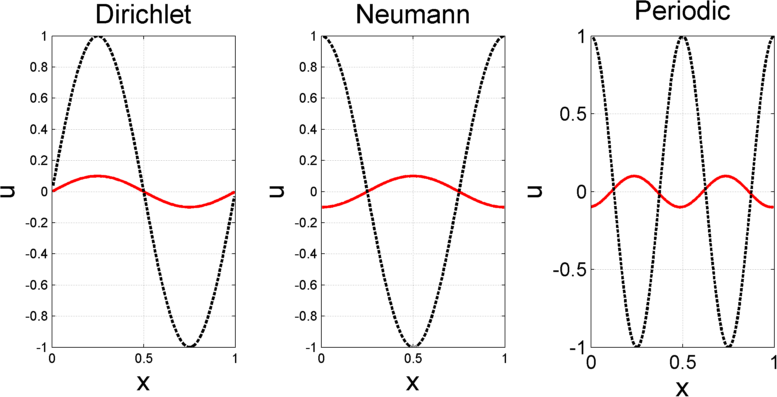
\includegraphics[width=\MeshFigWidth]{a06ex01EV2.png} 
		\caption{2nd Eigenvalue}
		\label{fig:a06ex01EV2}
	\end{subfigure}
	\begin{subfigure}[b]{0.5\hsize}
		\centering
		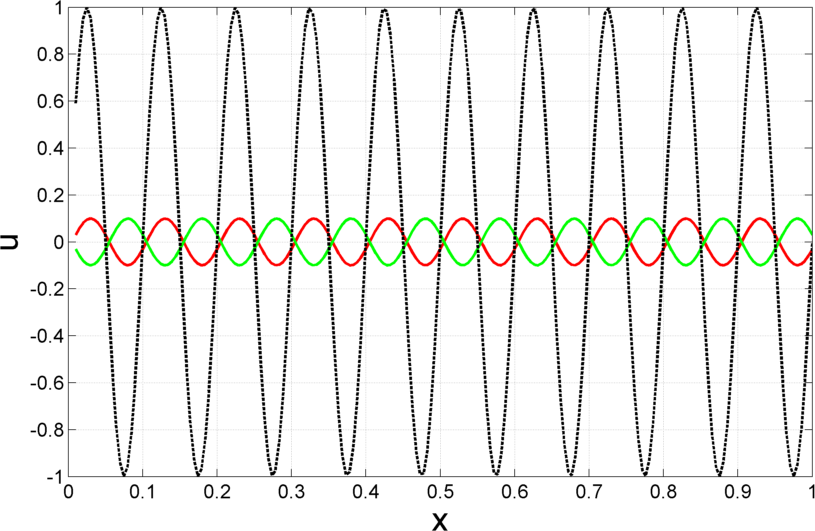
\includegraphics[width=\MeshFigWidth]{a06ex01EV20.png} 
		\caption{20th Eigenvalue}
		\label{fig:a06ex01EV20}
	\end{subfigure}
	\caption{Comparison of the Eigenvectors between discretized EV (black dashed), Dirichlet B.C. (red), Neumann B.C. (blue) and Periodic B.C. (green) for the 2nd and 20th Eigenvalue respectively.}
	\label{fig:a06ex01a}
\end{figure}
%
% ----------------
\addSubExercise{b}
Considering
\begin{align}
	-\Delta v &= \lambda v \;\text{ in } \Omega, \\
			v &= 0 		   \;\text{ on } \partial\Omega
\end{align}
with $\Omega = \{(x,y) \in \mathbb{R}^2 \colon \left(x-L/2\right)^2 + \left(y-L/2\right)^2 < R\}$ for given $L, R \in \mathbb{R}$ and $R>0$.
The Eigenvalues of such problem can be solved analytically utilizing the Bessel function of first kind $J_n(\xi)$ with $\xi = \sqrt{\lambda} R$ at its zero.
Taking the corresponding k-th zeros form the lecture notes, the first six Eigenvalues for $R=1$ and $R=2$  are stated in \TAB{a06ex01b}.
%
\vspace*{2\FigUpperVSpace}
\addTable{H}
		 {a06ex01b}
		 {First six Eigenvalues of the disc problem with respect to $R=1$ and $R=2$}
%
The solution was implemented in the form of a function submitted in \texttt{a06ex01\_solveEVPb.m}.
The function takes an arbitrary radius $R>0$ as input and gives the first six Eigenvalues and their $n$ values. 
%
% ----------------
\addSubExercise{c}
In this exercise, the domain $\Omega$ from assignment 5, exercise 1 has been discretized with respect to the disc problem in lecture notes with $L=2.2$ and $R=1$ and the the Laplace Operator $L_h$ has been built accordingly.
The numerical Eigenvalues have been numerically computed via reduced matrix $L_h$ for $h=1/(N+1)$ applied on three mesh resolutions with $N=7$, $N=63$, and $N=511$.
A comparison between the numerical and the exact Eigenvalues from \textbf{b)} is listed in \TAB{a06ex01c}.
The first four distinct eigenfunctions are demonstrated in \FIG{a06ex01c}.
For the implementation, please refer to online submitted \texttt{a06ex01\_solveEVPc.m} file.
%
\vspace*{2\FigUpperVSpace}
\addTable{H}
		 {a06ex01c}
		 {List of the first 6 Eigenvalues ordered by magnitude for different mesh resolution and the discretized analytical solution.}
%
\begin{figure}[H]
	\centering
	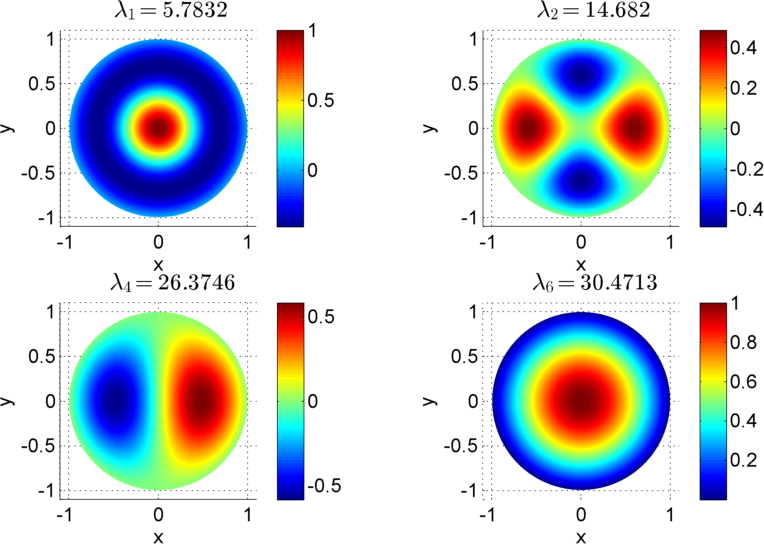
\includegraphics[width=0.9\textwidth]{a06ex01c.png} 
	\caption{Eigenfunctions of the first 4 distinct eigenvalues.
			 The value of the data has been respectively labeled with the color bar next to the plot.}
	\label{fig:a06ex01c}
\end{figure}
%
% EXERCISE 2
% --------------------------------------------------------------------------------------------------------------------
\addExercise{2}{Ex2}

% ----------------
\addSubExercise{a}
The discrete algorithm is implemented in a similar fashion to the one for section $II.5$ in the script, changing the lexicographic indexing to have the angle $\varphi$ vary over $i$ and $r$ over $j$. The operators are constructed in blocks by using Kronecker products of matrices containing the inverse radius coefficients for $\frac{1}{r_{ij}}\partial_{r}u_{ij}$ and $\frac{1}{r_{ij}^2}\partial_{\varphi\varphi}u_{ij}$. Multiplied with the corresponding adjacency matrices. The part a) and c) are thus jointly implemented in the program \listinline{a06ex02\_getPDE.py}

%
% ----------------
\addSubExercise{b}
We say the finite difference method is consistent if

\begin{equation*}
    \norm{f_h-L_h R_h u}_h \xrightarrow{ h \to 0} 0
\end{equation*}

Wlog let us take the maximum norm, that way we can write, by writing out the action of the restriction operator and the $L_h$ matrix:

\begin{equation*}
    max(f_h-L_hR_hu) \xrightarrow{ h \to 0} 0=
\end{equation*}

So lets consider the particular index $(ij)$ for which the maximal difference is reached, knowing that the difference stencil jumping considering neighbouring indices $j$ is the difference operator with respect to $r$ and the one considering neighbouring $i$ the one for $\varphi$

\begin{equation*}
    |(\partial_{rr}u_{ij}-D^{+}_jD^{-}_j)
    +\frac{1}{r_{ij}}(\partial_{r}u_{ij}-D^{0}_j)
    +\frac{1}{r_{ij}^2}(\partial_{\varphi\varphi}u_{ij}-D^{+}_iD^{-}_i)|
\end{equation*}

By the triangle inequality we can bound the expression by the sum of the maximums and take out the constant factors $\frac{1}{r_{ij}}$ and $\frac{1}{r_{ij}^2}$ since they are always positive.

\begin{equation*}
    |\partial_{rr}u_{ij}-D^{+}_jD^{-}_j|
    +\frac{1}{r_{ij}}|\partial_{r}u_{ij}-D^{0}_j|
    +\frac{1}{r_{ij}^2}|\partial_{\varphi\varphi}u_{ij}-D^{+}_iD^{-}_i|
\end{equation*}

Since we have the $r_{ij}\geq 1$ we can again bound by dropping the inverse factors in front of the last two summands. It is now clear that the total sum will tend to zero for small $h$, since all the differences are of order $O(h^2)$, so their sum will be too.

%
% ----------------
\addSubExercise{c}
\begin{figure}[H]
	\centering
	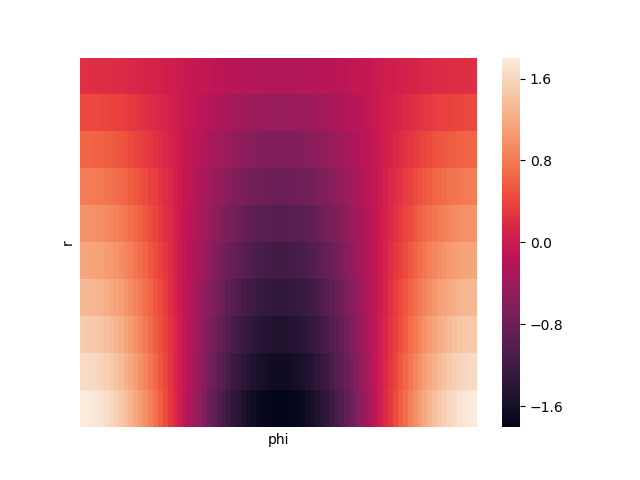
\includegraphics[width=0.9\textwidth]{Documentation/Figures/a06ex02c_uh.png} 
	\caption{}
	\label{fig:a06ex02c_uh}
\end{figure}

Figure \ref{fig:a06ex02c_uh} shows the plot of the anulus represented as a square in polar coordinates. Notice how the boundary values are satisfied at the upper and lower horizontal edges and how the periodicity condition holds across the left and right vertical ones.

The max error for the given $N_1$ and $N_2$ is 0.111

\begin{figure}[H]
	\centering
	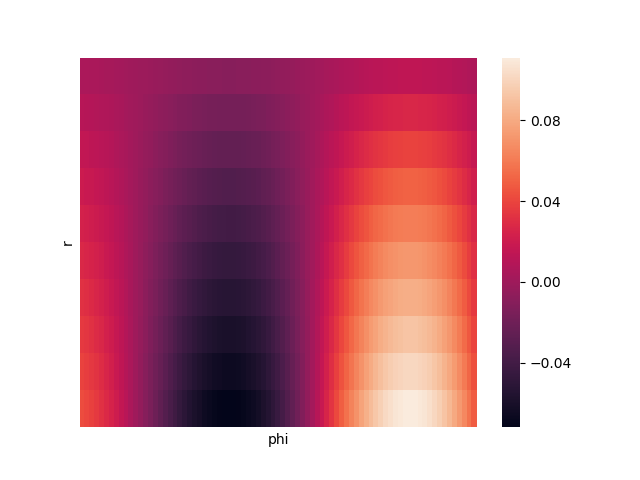
\includegraphics[width=0.9\textwidth]{Documentation/Figures/a06ex02c_error.png} 
	\caption{Error between the exact solution and the one obtained by the method in a). Notice the change in scale of the heat map}
	\label{fig:a05ex02b}
\end{figure}

\addSubExercise{d}

The error of this method is around 0.15 and does not seem to decrease with further refinement of the mesh. Another difference with respect to the method used in c is that here the discrete method consistently underestimates the solution, while in c) it is bot under and overestimated 

\begin{figure}[H]
	\centering
	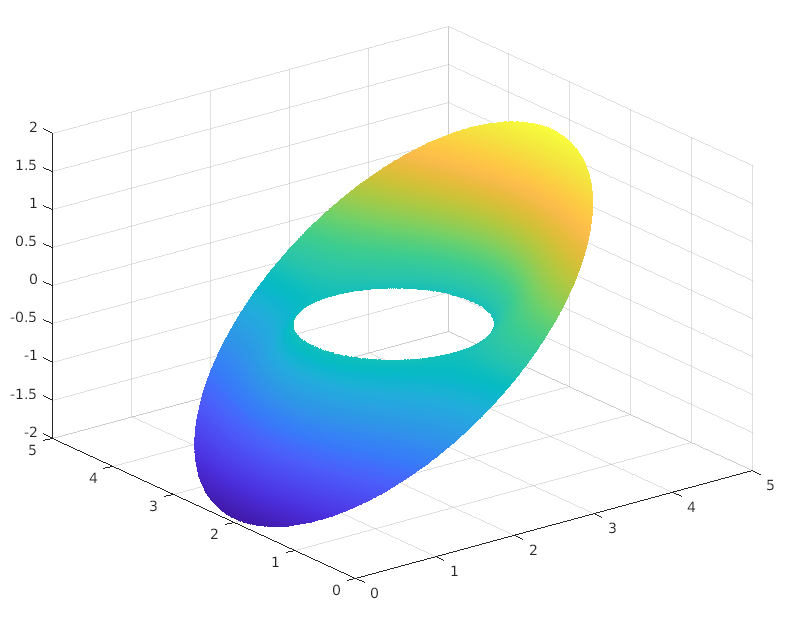
\includegraphics[width=0.9\textwidth]{Documentation/Figures/a06ex02d_uh.png} 
	\caption{Plot of the function values obtained using a modified version of the program from a05ex01}
	\label{fig:a05ex02b}
\end{figure}

\begin{figure}[H]
	\centering
	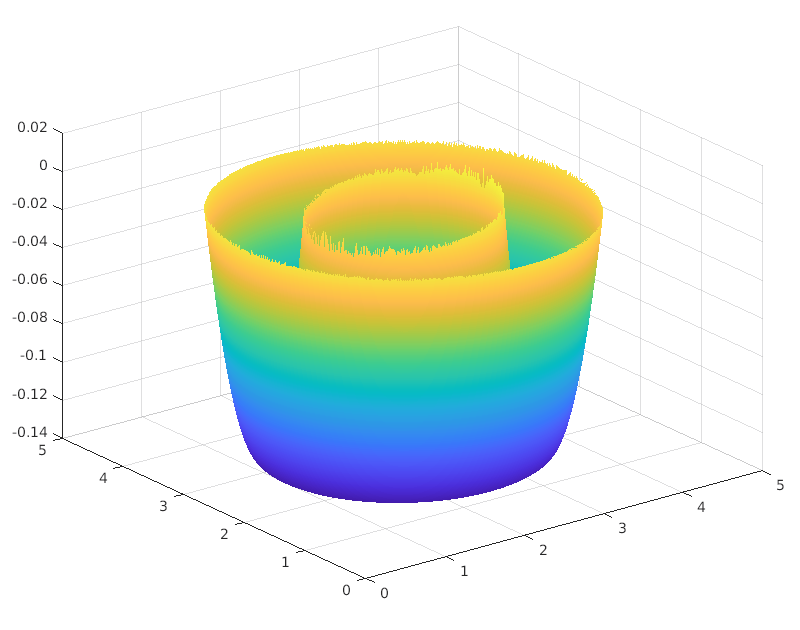
\includegraphics[width=0.9\textwidth]{Documentation/Figures/a06ex02d_error.png} 
	\caption{Error between the exact solution and the one obtained using a modified version of the program from a05ex01. Notice the change in scale of the vertical axis}
	\label{fig:a05ex02b}
\end{figure}
% EXERCISE 3
% --------------------------------------------------------------------------------------------------------------------
\addExercise{3}{Ex3}

\addSubExercise{a}
Please refer to the online submitted \texttt{a06e03getPDE.py} file.

\addSubExercise{b and c}

The grid size was empirically defined as $N = 20 + 10\sqrt{\varepsilon^{-1}}$.

\begin{figure}[H]
	\centering
	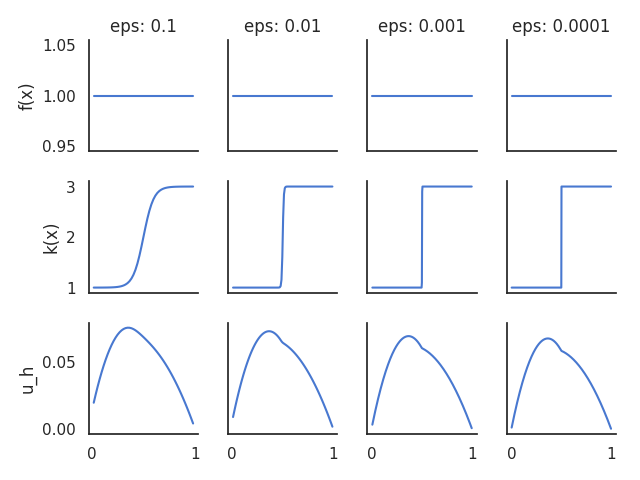
\includegraphics[width=0.68\textwidth]{a06e03plot.png}
	\caption{Functions $f(x)$, $k(x)$ and $u_h$ evaluated for $\varepsilon = 0.1, 0.01, 0.001, 0.0001$}
	\label{fig:a06e03plot}
\end{figure}

The function $k(x)$ will behave as a Heaviside step function for $\varepsilon \to 0$.